\documentclass{article}

\usepackage{amsmath}
\usepackage{amssymb}
\usepackage{amsbsy}
\usepackage{graphicx}
\usepackage{caption}
\usepackage{subcaption}
\usepackage{multirow}
\usepackage{placeins}

\graphicspath{{../images/}}

\let\bld\boldsymbol

\usepackage[backend=bibtex]{biblatex}
\bibliography{../hyparticle}

\author{Aditya Kashi}
\date{December 23, 2016}
\title{Numerical Analysis Project Report \\ \textbf{A particle method for conservation laws}}

\begin{document}
\maketitle

\begin{abstract}
An elegant particle method for the solution of one-dimensional scalar conservation laws is presented, following the development by Farjoun and Seibold \cite{particle}. The method is based on particle `management' based on conservation in the regions between the particles. Second-order accuracy is attained in both smooth regions and near shocks. The inviscid Burgers' equation is chosen here as the model problem to demonstrate the effectiveness of the method. However, extension to multi-dimensional problems and systems of conservation laws is not obvious.
\end{abstract}

\section{Introduction}
Background - numerical solution of conservation laws

State-of-the-practice (engineering): finite volume or finite difference methods with limiters, ENO/WENO or artificial dissipation terms.
\begin{itemize}
	\item second-order accurate only in smooth regions
	\item between first and second-order accurate at shocks
	\item TVD can usually be guaranteed only for scalar case
\end{itemize}
Based on `Eulerian' method, usually.


Solve scalar 1D conservation laws with a second-order TVD scheme.

\begin{align}
\frac{\partial u}{\partial t} + \frac{\partial f}{\partial x} = 0 \\
u(x,0) = u_0(x)
\label{eq:problem}
\end{align}

Burgers' equation: $f(u) = \frac{u^2}{2}$.
 

\section{The method}

The characteristic equations are key. \cite{particle}
\begin{align}
&\dot{x} = f'(u) \\
&\dot{u} = 0
\end{align}

The solution is a curve along which $u$ is constant, while $u$ is smooth. We can think in terms of `particles'.
 

Conservative particle management and interpolation

`Particle management' is needed when particles collide or get too far apart.
\begin{itemize}
	\item Based on local conservation of total `amount of $u$' between two particles.
	\item Rate of change of amount of $u$ contained between two particles
	\begin{equation}
		\frac{d}{dt}\int_{x_1(t)}^{x_2(t)}u(x,t)dx
	\end{equation}
	\item However, care must be taken because the limits of integration are now time-dependent.
\end{itemize}
 

After some calculation it can be shown, for space-independent flux functions $f$, that
\begin{equation}
\frac{d}{dt}\int_{x_1(t)}^{x_2(t)}u(x,t)dx = (x_2(t)-x_1(t))a_f(u_1,u_2)
\end{equation}
where
\begin{equation}
a_f(u_1,u_2) = \frac{[f'(u)-f(u)]_{u_1}^{u_2}}{[f'(u)]_{u_1}^{u_2}}.
\end{equation}
For Burgers' equation is
\begin{equation}
a_f(u_1,u_2) = \frac{u_1+u_2}{2}
\end{equation}

This is the basis of conservative particle management and conservative interpolation.
 
It has been shown that the method is second-order accurate away from shocks and TVD.

A `shock location' step has to be performed to achieve second-order accuracy in presence of shocks. However, for Burgers' equation, second order accuracy seems to be achieved irrespective of this.
 

\subsection{Implementation}
\begin{itemize}
	\item Since particles may need to be added or deleted anywhere, an array is not a good data structure. A linked list was coded, which allows efficient addition and deletion, at the cost of more expensive iteration through the particles.
	\item Conservative particle management is cheap only for quadratic flux functions. For others, a Newton iteration is required to solve for the new particles.
	\item Implementation in Julia programming language \cite{julia}
\end{itemize}

%\FloatBarrier

\section{Some results}

\begin{figure}
	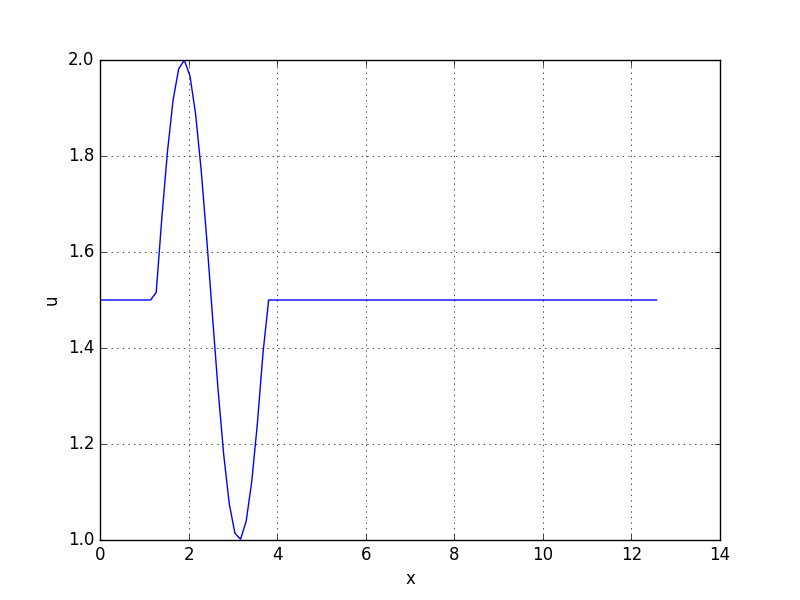
\includegraphics[scale=0.5]{hp-sol-n100-init}
	\caption{Initial condition}
\end{figure}
 

\begin{figure}
	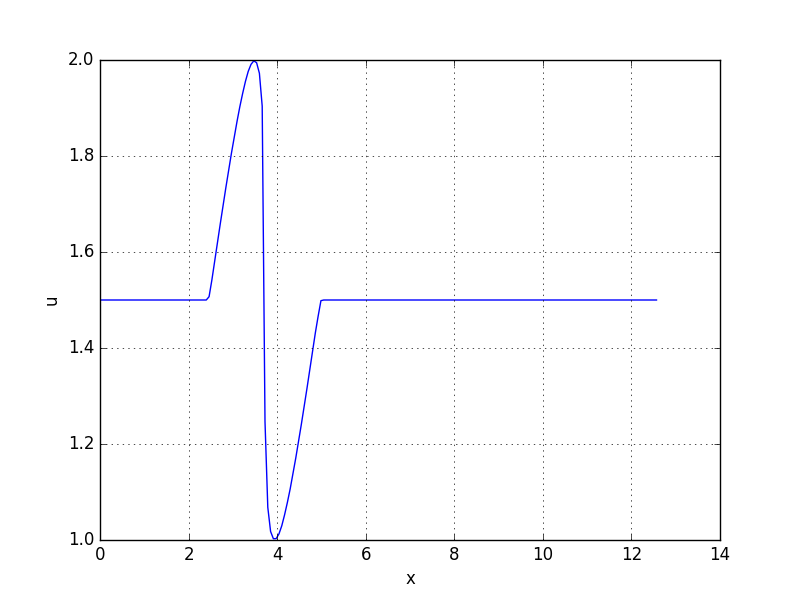
\includegraphics[scale=0.5]{hp-sol-t01}
	\caption{t = 0.1, before shock formation}
\end{figure}
 

\begin{figure}
	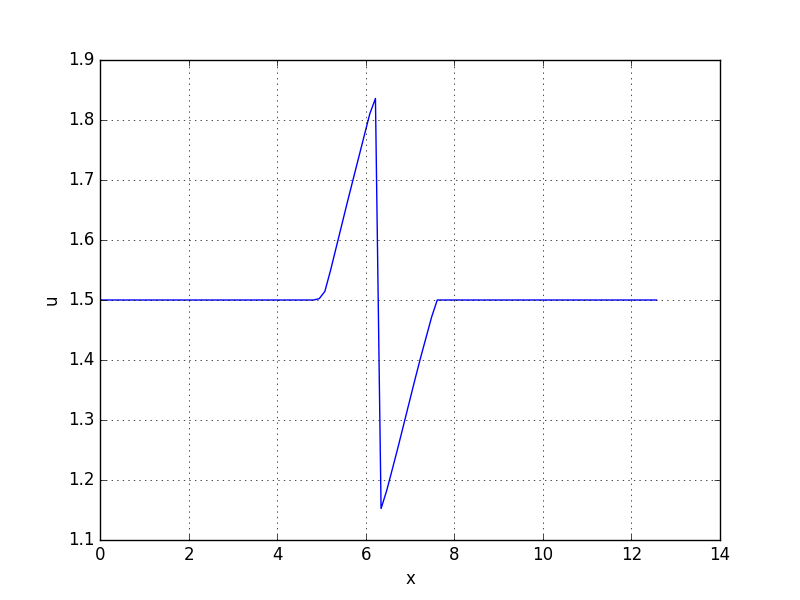
\includegraphics[scale=0.5]{hp-sol-n100-t25}
	\caption{t = 2.5, after shock formation}
\end{figure}
 
\begin{figure}
	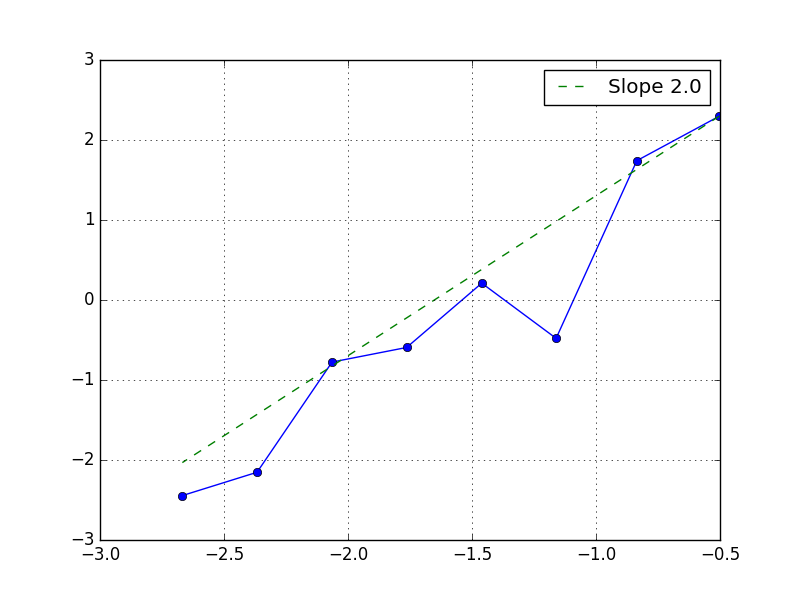
\includegraphics[scale=0.5]{hp-t25-grids8}
	\caption{Grid convergence for t = 2.5. The x axis is $\log_{10}||h||$, the y axis is $\log_{10}||u-u_{ref}||$}
\end{figure}
 
\begin{figure}
	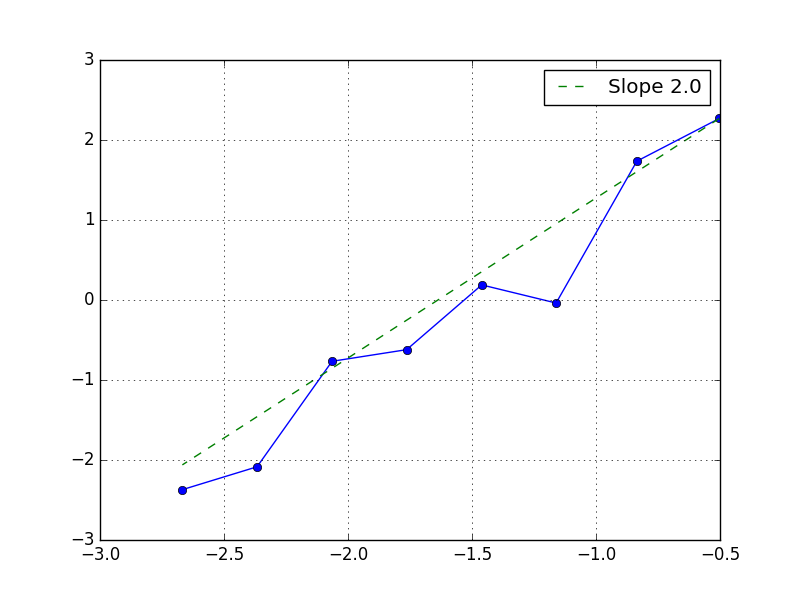
\includegraphics[scale=0.5]{hp-t25-nolocate}
	\caption{t = 2.5; no post-processing}
\end{figure}
 
%\FloatBarrier

\section{Conclusions and future work}

\begin{itemize}
	\item The particle method provides a way to achieve second-order accuracy for non-smooth solutions, at least for scalar conservation laws.
	\item An easy post-processing step is needed to maintain second-order accuracy in presence of shocks.
	\item However, extension to multi-dimensional problems and systems of conservation laws is not straightforward.
\end{itemize}
 

\subsection{Future work}

\subsubsection{Systems of conservation laws}
\begin{itemize}
	\item $\bld{f}'(\bld{u})$ is now a matrix with $N$ eigenvalues
	\item Speed of the particle?
	\item One possible solution: use $N$ different sets of particles.
	\item Can TVD still be guaranteed?
\end{itemize}
 

\subsubsection{Multidimensional problems}
\begin{itemize}
	\item In 1D, we have `next' and `previous' particles. Not so in multi-D.
	\item One could compute a Voronoi tessellation to get `neighbors' for each particle, and apply the 1D merge/insert for each pair thus generated.
	\item Implementation - data structures?
\end{itemize}
 

\subsubsection{Others}
\begin{itemize}
	\item Steady-state solutions?
	\item Implicit time stepping?
\end{itemize}
 

\printbibliography

\end{document}